\section{Lineare Regression}
    In einem Versuchteil wurden die folgenden Daten für Liniennummer $N_{Linie}$
    und Spannung $U$ aufgenommen.
    Die Liniennummern $N_{Linie}$ sollen dabei gemäß der Formel \ref{eqn:formel} in die Abstände $D$ umgerechnet werden. 
    \begin{equation}
        D=(N_{Linie}-1) \cdot 6 \si{mm.}
        \label{eqn:formel}
    \end{equation}

    \begin{table}[H]
        \centering
        \begin{tabular}{c c c}
            \toprule
            Liniennummer $N_{Linie}$ & $U\;/\;$V & $D\;/\;$mm \\
            \midrule
            1&-19.5&0\\
            2&-16.1&6\\
            3&-12.4&12\\
            4&-9.6&18\\
            5&-6.2&24\\
            6&-2.4&30\\
            7&1.2&36\\
            8&5.1&42\\
            9&8.3&48\\
            \bottomrule
        \end{tabular}
        \caption{Messdaten, Liniennummer $N_{Linie}$ und Spannung $U$ mit berechneten
            Abständen $D$ nach Gl. \ref{eqn:formel}}
        \label{tab:tabelle}
    \end{table}

    Trägt man nun die Spannung $U$ gegen den Abstand $D$ auf, so folgt für eine lineare 
    Regression nach 
    \begin{equation}
        U=m\cdot D + n,
        \label{eqn:gerade}
    \end{equation}
    für die Steigung $m$ und den y-Achsenabschnitt $n$
    \begin{align*}
        m&=(0.581\pm0.007) \si{\volt\per\mm},\\
        n&=(-19.68\pm0.19) \si{V}.\\
    \end{align*}
    \begin{figure}[H]
        \centering
        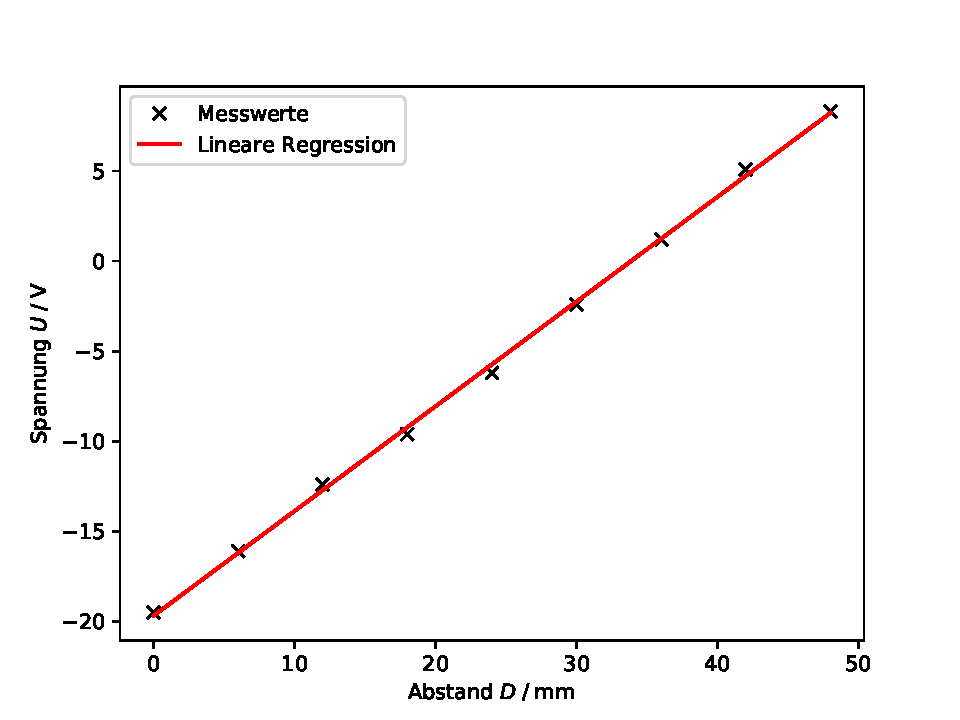
\includegraphics[width=0.8\textwidth]{plot.pdf}
        \caption{In der Grafik wird die Spannung $U$ gegen den Abstand $D$ aufgetragen, sowie 
        die lineare Regression nach der Geradengleichung \ref{eqn:gerade} mit derer Parameter.}
    \end{figure}